% Created 2017-02-13 Mon 17:52
% Intended LaTeX compiler: pdflatex
\documentclass[presentation,smaller]{beamer}
\RequirePackage{etex}
\RequirePackage[l2tabu,orthodox]{nag}            %% Warn about obsolete commands and packages
\RequirePackage{amsmath,amsfonts,amssymb,amsthm} %% Math
\RequirePackage{ifxetex,ifluatex}                %% Detect XeTeX and LuaTeX
\RequirePackage{fixltx2e}                        %% provides \textsubscript
\RequirePackage{xspace}
\RequirePackage{graphicx}
\RequirePackage{comment}
\RequirePackage{url}
\RequirePackage{relsize}
\RequirePackage{booktabs}
\RequirePackage{tabularx}
\RequirePackage[normalem]{ulem}
\RequirePackage[all]{xy}
\RequirePackage{etoolbox}

%%%
%%% Code Listings
%%%

\RequirePackage{listings}
\lstdefinelanguage{Sage}[]{Python}{morekeywords={True,False,sage,cdef,cpdef,ctypedef,self},sensitive=true}

\lstset{frame=none,
  showtabs=False,
  showspaces=False,
  showstringspaces=False,
  commentstyle={\color{gray}},
  keywordstyle={\color{mLightBrown}\textbf},
  stringstyle ={\color{mDarkBrown}},
  frame=single,
  basicstyle=\tt\scriptsize\relax,
  backgroundcolor=\color{gray!190!black},
  inputencoding=utf8,
  literate={…}{{\ldots}}1,
  belowskip=0.0em,
}

\makeatletter
\patchcmd{\@verbatim}
  {\verbatim@font}
  {\verbatim@font\scriptsize}
  {}{}
\makeatother

%%%
%%% Tikz
%%%

\RequirePackage{tikz,pgfplots}

\usetikzlibrary{calc}
\usetikzlibrary{arrows}
\usetikzlibrary{automata}
\usetikzlibrary{positioning}
\usetikzlibrary{decorations.pathmorphing}
\usetikzlibrary{backgrounds}
\usetikzlibrary{fit,}
\usetikzlibrary{shapes.symbols}
\usetikzlibrary{chains}
\usetikzlibrary{shapes.geometric}
\usetikzlibrary{shapes.arrows}
\usetikzlibrary{graphs}

%% Cache

\ifdefined\tikzcaching  % chktex 1
  \usetikzlibrary{external}
  \tikzexternalize[prefix=build/]
  \tikzset{external/up to date check=diff}  %% MD5 fails from within emacs
\fi

%%%
%%% SVG (Inkscape)
%%%

\ifxetex % chktex 1
\newcommand{\executeiffilenewer}[3]{%
  {\immediate\write18{#3}} % hack
}
\else
\newcommand{\executeiffilenewer}[3]{%
  \ifnum\pdfstrcmp{\pdffilemoddate{#1}}%
    {\pdffilemoddate{#2}}>0%
    {\immediate\write18{#3}}
  \fi%
}
\fi

\newcommand{\includesvg}[2][1.0\textwidth]{%
 \executeiffilenewer{#1.svg}{#1.pdf}%
 {inkscape -z -D --file=#2.svg --export-pdf=#2.pdf --export-latex --export-area-page}%
 \def\svgwidth{#1} 
 \input{#2.pdf_tex}%
} 

%%%
%%% Metropolis Theme
%%%

\usetheme{metropolis}
\metroset{color/block=fill}
\metroset{numbering=none}
\metroset{outer/progressbar=foot}
\metroset{titleformat=smallcaps}

\setbeamercolor{description item}{fg=mLightBrown}
% \setbeamerfont{alerted text}{series=\bfseries}
\setbeamerfont{footnote}{size=\scriptsize}
\setbeamercolor{example text}{fg=mDarkBrown}

\renewcommand*{\UrlFont}{\ttfamily\smaller\relax}

%%%
%%% UTF-8
%%% 

\RequirePackage{unicodesymbols} % after metropolis which loads fontspec

%%%
%%% BibLaTeX
%%%

\RequirePackage[backend=bibtex,
            style=alphabetic,
            maxnames=4,
            citestyle=alphabetic]{biblatex}

\bibliography{local.bib,abbrev3.bib,crypto_crossref.bib,rfc.bib,jacm.bib}

\DeclareFieldFormat{title}{\alert{#1}}
\DeclareFieldFormat[book]{title}{\alert{#1}}
\DeclareFieldFormat[thesis]{title}{\alert{#1}}
\DeclareFieldFormat[inproceedings]{title}{\alert{#1}}
\DeclareFieldFormat[incollection]{title}{\alert{#1}}
\DeclareFieldFormat[article]{title}{\alert{#1}}
\DeclareFieldFormat[misc]{title}{\alert{#1}}

%%% 
%%% Microtype
%%%

\IfFileExists{upquote.sty}{\RequirePackage{upquote}}{}
\IfFileExists{microtype.sty}{\RequirePackage{microtype}}{}

\setlength{\parindent}{0pt}                   %%
\setlength{\parskip}{6pt plus 2pt minus 1pt}  %%
\setlength{\emergencystretch}{3em}            %% prevent overfull lines
\setcounter{secnumdepth}{0}                   %%

%%% Local Variables:
%%% mode: latex
%%% End:
\usepackage{graphicx}
\usepackage{grffile}
\usepackage{longtable}
\usepackage{wrapfig}
\usepackage{rotating}
\usepackage[normalem]{ulem}
\usepackage{amsmath}
\usepackage{textcomp}
\usepackage{amssymb}
\usepackage{capt-of}
\usepackage{hyperref}
\usepackage{microtype}
\usepackage{newunicodechar}
\usepackage[notions,operators,sets,keys,ff,adversary,primitives,complexity,asymptotics,lambda,landau,advantage]{cryptocode}
\usepackage{xspace}
\usepackage{units}
\usepackage{nicefrac}
\usepackage{gensymb}
\usepackage{amsthm}
\usepackage{amsmath}
\usepackage{amssymb}
\usepackage{xcolor}
\usepackage{listings}
\usepackage[color=yellow!40]{todonotes}
\renewcommand{\vec}[1]{\mathbf{#1}\xspace}
\newcommand{\mat}[1]{\mathbf{#1}\xspace}
\DeclareMathOperator{\Vol}{Vol}
\usetheme{default}
\author{Martin R. Albrecht}
\date{Oxford Lattice School}
\title{Attacks on LWE}
\hypersetup{
pdfauthor={Martin R. Albrecht},
pdftitle={Attacks on LWE},
pdfkeywords={},
pdfsubject={},
pdfcreator={Emacs 25.1.1 (Org mode 9.0.4)},
pdflang={English},
colorlinks,
citecolor=gray,
filecolor=gray,
linkcolor=gray,
urlcolor=gray
}
\begin{document}

\maketitle
\begin{frame}{Outline}
\tableofcontents
\end{frame}


\section{BKZ}
\label{sec:org25d5b1a}
\begin{frame}[label={sec:org6fe0067}]{BKZ}
\begin{itemize}
\item Input basis is LLL reduced, the \alert{first block} is \(\vec{b}_1,\dots,\vec{b}_{β}\).
\item Call the SVP oracle to obtain a short vector, \(\vec{b}_1'\), in the space spanned by these vectors.
\item Now have \(β+1\) vectors spanning a \(β\) dimensional space, call LLL to obtain a set of \(β\) linearly independent vectors.
\item The \alert{second block} is made of vectors which are the projection of \(\vec{b}_2,\dots, \vec{b}_{β+1}\) onto the space which is orthognal to \(\vec{b}_1\).
\item Again, call SVP oracle to obtain a short vector in this space, \(\vec{b}_2'\), which can be viewed as the projection of some \(\vec{b}_2''\) in the lattice.
\item Call LLL on \(\vec{b}_2, \vec{b}_3,\dots, \vec{b}_{β+1}, \vec{b}_2''\) to update the list of basis vectors.
\end{itemize}

… start again when reaching end, repeat until nothing changes
\end{frame}

\begin{frame}[label={sec:orgbce9e22}]{BKZ 2.0}
\begin{description}
\item[{early abort}] BKZ eventually terminates when there is nothing left to do. However, most work is done in the first few tours
\item[{recursive preprocessing}] use BKZ with smaller block size to preprocess blocks before calling the SVP oracle
\item[{(extreme) pruning}] choose pruning parameters which lead to low probability of success, rerandomise and repeat to boost probability
\item[{Gaussian heuristic}] use the Gaussian heuristic to set radius for enumeration search
\end{description}

\begin{block}{}
\fullcite{PhD:Chen13}, implementation: \url{https://github.com/fplll/fplll}
\end{block}
\end{frame}

\begin{frame}[label={sec:orgb907b2e}]{root-Hermite Factors}
\begin{itemize}
\item Hermite factor: \(δ_0^n\)
\item root-Hermite factor:  \(δ_0\)
\item log root-Hermite factor: \(\log_2 δ_0\)
\end{itemize}

The shortest non-zero vector \(\vec{b}_1\) in the output basis satisfies: \[\|\vec{b}_1\| = δ_0^n⋅ \Vol(Λ)^{1/n}.\]
\end{frame}

\begin{frame}[label={sec:org3925836}]{Gaussian Heuristic}
Let \(Λ \subset \ZZ^n\) be a lattice and let \(S \in \mathbb{R}^n\) be a measurable subset of the real space. Then \[|S ∩ Λ| ≈ \Vol(S)/\Vol(Λ).\]

As a corollary, considering spheres, we get: \[λ_1(Λ) ≈ \sqrt{\frac{n}{2 π e}} \Vol(Λ)^{1/n}.\]
\end{frame}

\begin{frame}[label={sec:org8cad765}]{Geometric Series Assumption}
The norms of the Gram-Schmidt vectors after lattice reduction satisfy \footfullcite{STACS:Schnorr03} \[\|b_i^*\| = α^{i-1} ⋅ \|\vec{b}_1\| \textnormal{ for some } 0 < α < 1.\]

Combining this with the root-Hermite factor \(\|\vec{b}_1\| = δ_0^n \Vol(Λ)^{1/n}\) and \(\Vol(Λ) = \prod_{i=1}^{n} \|b_i^*\|\), we get \[α = δ^{-2n/(n-1)}.\] 
\end{frame}

\begin{frame}[label={sec:orgc36fc4b}]{BKZ Quality}
Assuming the \alert{Gaussian Heuristic} (GH) and the \alert{Geometric Series Assumption} (GSA), a limiting value of the root-Hermite factor \(δ_0\) achievable by BKZ is \footfullcite{PhD:Chen13}: \[\lim_{n \rightarrow \infty} δ_0 = \left(v_β^{\frac{-1}{β}}\right)^{\frac{1}{β-1}}  ≈  \left( \frac{β}{2 \pi e} (\pi β)^{\frac{1}{β}}  \right)^{\frac{1}{2(β-1)}}\]

where \(v_β\) is the volume of the unit ball in dimension \(β\). Experimental evidence suggests that we may apply this as an estimate for \(\delta_0\) also in practice.
\end{frame}

\begin{frame}[label={sec:orgaf18df8}]{BKZ Quality}
\begin{tikzpicture}
\pgfplotsset{width=\textwidth, height=0.6\textwidth}

\begin{axis}[xlabel={$\beta$},ylabel={$\delta_0$},legend pos=north east, legend style={fill=none},  yticklabel style={/pgf/number format/fixed, /pgf/number format/precision=4}]
         	
\addplot[black, thick] coordinates {
(50, 1.01206486355485) (60, 1.01145310214785) (70, 1.01083849117278)
(80, 1.01026264533039) (90, 1.00973613406057) (100, 1.00925872103633)
(110, 1.00882653150498) (120, 1.00843474281592) (130, 1.00807860284815)
(140, 1.00775378902354) (150, 1.00745650119215) (160, 1.00718344897388)
(170, 1.00693180103572) (180, 1.00669912477197) (190, 1.00648332800111)
(200, 1.00628260691082) (210, 1.00609540127612) (220, 1.00592035664374)
(230, 1.00575629268952) (240, 1.00560217684407) (250, 1.00545710232739)
};
\addlegendentry{$(\frac{\beta}{2\pi e} \cdot (\pi\, \beta)^{1/\beta} )^{\frac{1}{2(\beta-1)}}$};

\end{axis}
\end{tikzpicture}
\end{frame}

\begin{frame}[label={sec:org6a1cd6c}]{Running Time}
\begin{center}
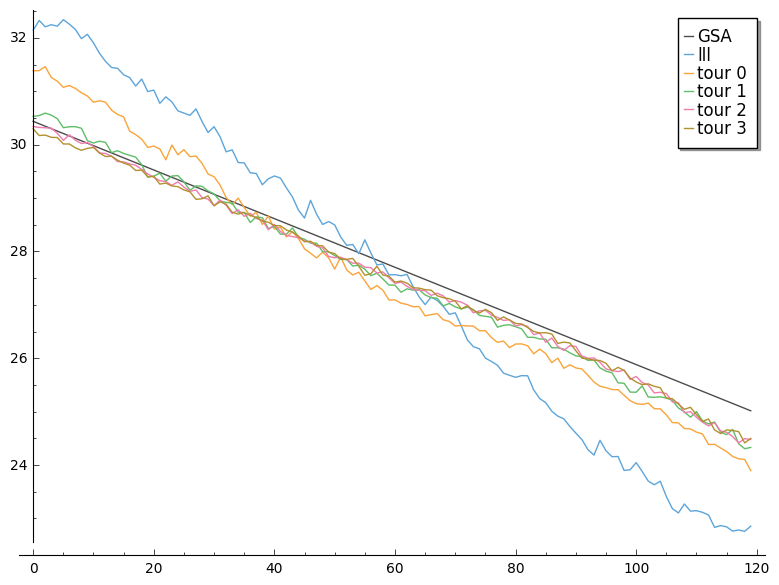
\includegraphics[width=0.8\textwidth]{bkz-quality.png}
\end{center}

Most work is done in first 3-4 tours.
\end{frame}

\begin{frame}[label={sec:orgb37ab4d}]{Running Time}
Per tour, BKZ calls 
\begin{description}
\item[{\(c_{\textnormal{pre},β}\)}] prepare \(n\) SVP calls
\item[{\(c_{\textnormal{svp},β}\)}] \(n\) SVP oracle calls in block size \(≤ β\)
\item[{\(c_{\textnormal{lll}}\) }] \(n\) LLL calls to insert the vector into the basis
\end{description}

Total cost: \[≈ 4\,n \cdot (c_{\textnormal{pre},β} + c_{\textnormal{svp},β} + c_{\textnormal{lll}})\]
\end{frame}

\begin{frame}[label={sec:orgc27472c}]{Running Time}
We assume 
\begin{itemize}
\item \(c_{\textnormal{pre},β} < c_{\textnormal{svp},β}\)\footnote{For current code, this is a bold lie.} and
\item \(c_{\textnormal{lll}} \ll c_{\textnormal{svp},β}\)
\end{itemize}
to obtain \[≈ 4\,n\, c_{\textnormal{svp},β}\]

Asymptotically, sieving is the most efficient heuristic SVP algorithm, with a cost \footfullcite{SODA:BDGL16} of \[c_{\textnormal{svp},β} = 2^{0.292\,β + o(1)}.\]
\end{frame}

\begin{frame}[label={sec:orgd029702}]{Asymptotic Behaviour}
The log of the time complexity for running BKZ to achieve a root-Hermite factor \(\delta_0\) is:

\begin{eqnarray*}
\Omega \left( \frac{-\log\left(\frac{-\log\log \delta_0}{\log \delta_0}\right) \log\log\delta_0}{\log\delta_0} \right) & & \textnormal{for enumeration},\\
\Omega \left( \frac{-\log\log \delta_0}{\log\delta_0} \right) & & \textnormal{for sieving}.
\end{eqnarray*}
\end{frame}

\section{LWE}
\label{sec:org8cdbedc}
\begin{frame}[label={sec:org95f1879}]{Learning with Errors}
Let \(n,\,q\) be positive integers, \(\chi\) be a probability distribution on \(\ZZ\) and \(\vec{s}\) be a secret vector in \(\ZZ_q^n\). We denote by \(L_{n,q,\chi}\) the probability distribution on \(\ZZ_q^n × \ZZ_q\) obtained by choosing \(\vec{a} ∈ \ZZ_q^n\) uniformly at random, choosing \(e ∈ \ZZ\) according to χ and considering it in \(\ZZ_q\), and returning \((\vec{a}, c) = (\vec{a}, \Angle{\vec{a},\vec{s}}+ e) ∈ \ZZ_q^n × \ZZ_q\).

\begin{description}
\item[{Decision-LWE}] is the problem of deciding whether pairs \((\vec{a}, c) ∈ \ZZ_q^n × \ZZ_q\) are sampled according to \(L_{n, q, \chi}\) or the uniform distribution on \(\ZZ_q^n × \ZZ_q\).

\item[{Search-LWE}] is the problem of recovering \(\vec{s}\) from \((\vec{a}, c)=(\vec{a}, \Angle{\vec{a},\vec{s}} + e) ∈ \ZZ_q^n × \ZZ_q\) sampled according to \(L_{n, q, \chi}\).
\end{description}
\end{frame}

\section{Dual Lattice Attack}
\label{sec:org4aac7b6}
\begin{frame}[label={sec:org66cc163}]{Short Integer Solutions}
Consider the scaled (by \(q\)) dual lattice: \[q Λ^* = \{ \vec{x} \in \mathbb{Z}^m \enspace | \enspace \vec{x} \vec{A} \equiv 0 \bmod q\}.\] A short vector of \(qΛ^*\) is equivalent to solving SIS on \(\vec{A}\).

\begin{block}{Short Integer Solutions (SIS)}
Given \(q \in \mathbb{Z}\), a matrix \(\vec{A}\), and \(t < q\); find \(\vec{y}\) with \(0 < \|\vec{y}\| \leq t\) and \[\vec{y}\, \vec{A} \equiv  \vec{0} \pmod{q}.\]
\end{block}
\end{frame}

\begin{frame}[label={sec:org11e6e4c}]{Strategy}
\begin{itemize}
\item Given LWE samples \(\vec{A}, \vec{c}\) where either \(\vec{c} = \vec{A}\vec{s} + \vec{e}\) or \(\vec{c}\) uniformly random.
\item Find a short \(\vec{y}\) solving SIS on \(\vec{A}\).
\item Compute \(\Angle{\vec{y}, \vec{c}}\). 
\begin{itemize}
\item If \(\vec{c} = \vec{A} \cdot \vec{s} + \vec{e}\), then \(\Angle{\vec{y}, \vec{c}} = \Angle{\vec{y}\vec{A}, \vec{s}} + \Angle{\vec{y}, \vec{e}} \equiv \Angle{\vec{y}, \vec{e}} \pmod{q}\).
\item If \(\vec{c}\) is uniformly random, so is \(\Angle{\vec{y}, \vec{c}}\).
\end{itemize}
\end{itemize}

If \(\vec{y}\) is sufficiently short, then \(\Angle{\vec{y}, \vec{e}}\) will also be short, since \(\vec{e}\) is also small, and can be distinguished from uniform values.
\end{frame}

\begin{frame}[label={sec:orgd8fba33}]{Required Quality}
Given an LWE instance characterised by \(n\), \(α\), \(q\) and a vector \(\vec{v}\) of length \(\|\vec{v}\|\) in the scaled dual lattice \[qΛ^* = \{ \vec{w} \in \ZZ_q^m \ | \ \vec{w} ⋅  \vec{A} \equiv 0 \bmod{q} \},\] the advantage of distinguishing \(\Angle{\vec{v},\vec{e}}\) from random is close to \[\exp\left(-π (\|\vec{v}\| \cdot α)^2\right).\]
\end{frame}

\begin{frame}[label={sec:org9d6cb68}]{Lattice Reduction}
A reduced lattice basis is made of short vectors, in particular the first vector has norm \(δ_0^m \cdot \Vol(qΛ^*)^{1/m}\)
\begin{itemize}
\item Construct a basis of the dual from the instance.
\item Feed to a lattice reduction algorithm to obtain short vectors \(\vec{v}_i\).
\item Check if \(\vec{v}_i\, \vec{A}\) are small.
\end{itemize}
\end{frame}

\begin{frame}[label={sec:org2e29b27}]{Constructing a Basis}
\begin{itemize}
\item We seek a basis for the \(q\)-ary lattice \[qΛ^* = \{ \vec{w} \in \ZZ_q^m \ | \ \vec{w}⋅ \vec{A} \equiv 0 \bmod{q} \}\]
\item Compute a row-echelon form \(\mat{Y}\) of the basis for the left-kernel of \(\vec{A}\) using Gaussian elimination.
\item With high probability it will have dimension \((m-n) × m\)
\item Write \(\mat{Y} = [\vec{I}_{(m-n) \times (m-n)} | \mat{Y}']\)
\item Extend to \(q\)-ary lattice by stacking with  \([\vec{0}_{n \times (m-n)} \mid q ⋅ \vec{I}_{n \times n}]\)
\item Our basis is:
\begin{align*}
  \mat{L} = \begin{pmatrix}
    \mat{I}_{(m-n) \times (m-n)} & \mat{Y}'\\
    0 & q\, \mat{I}_{n \times n}
  \end{pmatrix}
\end{align*}
\end{itemize}
\end{frame}

\begin{frame}[label={sec:org01373cc}]{Degrees of Freedom}
We get to choose:

\begin{itemize}
\item the dimension \(m\), i.e. the number of samples we use
\item the target advantage \(ε\) for distinguishing
\end{itemize}
\end{frame}

\begin{frame}[label={sec:orgee715d5}]{Choosing \(m\)}
Example: \(q=2^{17}, n=1024, δ_0 = 1.005\)

\begin{tikzpicture}
\pgfplotsset{width=1.0\textwidth, height=0.5\textwidth}

\begin{axis}[xlabel={$m$},ylabel={$\log_2 δ_0^m \cdot q^{n/m}$},legend pos=north east, legend style={fill=none},  yticklabel style={/pgf/number format/fixed, /pgf/number format/precision=4}]
         	
\addplot[black, thick] coordinates {
(1024, 24.3681934379047) (1040, 24.2217829988335) (1056, 24.0832979676877) (1072, 23.9523834754557)
(1088, 23.8287055277737) (1104, 23.7119494922699) (1120, 23.6018187155654) (1136, 23.4980332571473)
(1152, 23.4003287287538) (1168, 23.3084552291511) (1184, 23.2221763652800) (1200, 23.1412683517112)
(1216, 23.0655191811960) (1232, 22.9947278598492) (1248, 22.9287037011642) (1264, 22.8672656736477)
(1280, 22.8102417973808) (1296, 22.7574685852802) (1312, 22.7087905252422) (1328, 22.6640595997224)
(1344, 22.6231348396308) (1360, 22.5858819097171) (1376, 22.5521727228821) (1392, 22.5218850810884)
(1408, 22.4949023407553) (1424, 22.4711131007098) (1440, 22.4504109109423) (1456, 22.4326940005646)
(1472, 22.4178650235097) (1488, 22.4058308206380) (1504, 22.3965021970288) (1520, 22.3897937133371)
(1536, 22.3856234901903) (1552, 22.3839130246851) (1568, 22.3845870181180) (1584, 22.3875732141578)
(1600, 22.3928022467260) (1616, 22.4002074969161) (1632, 22.4097249583272) (1648, 22.4212931102443)
(1664, 22.4348527981335) (1680, 22.4503471209671) (1696, 22.4677213249258) (1712, 22.4869227030623)
(1728, 22.5079005005382) (1744, 22.5306058250782) (1760, 22.5549915623077) (1776, 22.5810122956677)
(1792, 22.6086242306189) (1808, 22.6377851228712) (1824, 22.6684542103905) (1840, 22.7005921489523)
(1856, 22.7341609510298) (1872, 22.7691239278147) (1888, 22.8054456341876) (1904, 22.8430918164611)
(1920, 22.8820293627379) (1936, 22.9222262557286) (1952, 22.9636515278910) (1968, 23.0062752187576)
(1984, 23.0500683343274) (2000, 23.0950028084075) (2016, 23.1410514657954) (2032, 23.1881879872003)
};
\end{axis}
\end{tikzpicture}

\[m = \sqrt{\frac{n\,\log q}{\log(\delta_0)}}\]
\end{frame}

\begin{frame}[label={sec:orgb34d253}]{Choosing \(ε\)}
\begin{tikzpicture}
\pgfplotsset{width=1.0\textwidth, height=0.5\textwidth}

\begin{axis}[xlabel={$\varepsilon = 1/2^i$},ylabel={\(\log_2\left(\textnormal{BKZ cost}\right)\)},legend pos=north east, legend style={fill=none},  yticklabel style={/pgf/number format/fixed, /pgf/number format/precision=4}]
         	
\addplot[black, thick] coordinates {
( 1, 410.3) ( 2, 374.0) ( 3, 355.0) ( 4, 342.4)
( 5, 333.1) ( 6, 325.5) ( 7, 319.6) ( 8, 314.4)
( 9, 310.0) (10, 305.9) (11, 302.7) (12, 299.4)
(13, 296.5) (14, 293.9) (15, 291.5) (16, 289.5)
(17, 287.4) (18, 285.4) (19, 283.6) (20, 282.2)
(21, 280.4) (22, 279.0) (23, 277.5) (24, 276.0)
(25, 274.9) (26, 273.7) (27, 272.5) (28, 271.4)
(29, 270.2) (30, 269.3) (31, 268.1) (32, 267.3)
(33, 266.4) (34, 265.5) (35, 264.6) (36, 263.7)
(37, 262.9) (38, 262.3) (39, 261.4) (40, 260.5)
(41, 259.9) (42, 259.4) (43, 258.5) (44, 257.9)
(45, 257.3) (46, 256.7) (47, 256.1) (48, 255.6)
(49, 255.0) (50, 254.4) (51, 253.8) (52, 253.2)
(53, 252.6) (54, 252.0) (55, 251.7) (56, 251.2)
(57, 250.6) (58, 250.3) (59, 249.7) (60, 249.1)
(61, 248.8) (62, 248.2) (63, 247.9)
};
\end{axis}
\end{tikzpicture}
\end{frame}

\begin{frame}[label={sec:orgc94eeda}]{Choosing \(ε\)}
Boost the advantage to constant, repeat experiment \(≈ 1/ε^2\) times

\begin{tikzpicture}
\pgfplotsset{width=1.0\textwidth, height=0.5\textwidth}

\begin{axis}[xlabel={$\varepsilon = 1/2^i$},ylabel={\(\log_2\left( 2^{2\,i} \cdot \textnormal{BKZ cost}\right)\)},legend pos=north east, legend style={fill=none},  yticklabel style={/pgf/number format/fixed, /pgf/number format/precision=4}]
         	
\addplot[black, thick] coordinates {
( 1, 412.3) ( 2, 378.0) ( 3, 361.0) ( 4, 350.4)
( 5, 343.1) ( 6, 337.5) ( 7, 333.6) ( 8, 330.4)
( 9, 328.0) (10, 325.9) (11, 324.7) (12, 323.4)
(13, 322.5) (14, 321.9) (15, 321.5) (16, 321.5)
(17, 321.4) (18, 321.4) (19, 321.6) (20, 322.2)
(21, 322.4) (22, 323.0) (23, 323.5) (24, 324.0)
(25, 324.9) (26, 325.7) (27, 326.5) (28, 327.4)
(29, 328.2) (30, 329.3) (31, 330.1) (32, 331.3)
(33, 332.4) (34, 333.5) (35, 334.6) (36, 335.7)
(37, 336.9) (38, 338.3) (39, 339.4) (40, 340.5)
(41, 341.9) (42, 343.4) (43, 344.5) (44, 345.9)
(45, 347.3) (46, 348.7) (47, 350.1) (48, 351.6)
(49, 353.0) (50, 354.4) (51, 355.8) (52, 357.2)
(53, 358.6) (54, 360.0) (55, 361.7) (56, 363.2)
(57, 364.6) (58, 366.3) (59, 367.7) (60, 369.1)
(61, 370.8) (62, 372.2) (63, 373.9)};
\end{axis}
\end{tikzpicture}
\end{frame}

\begin{frame}[label={sec:org6614e2c}]{Amortising Costs}
Our discussion on choosing \(ε\) was based on the assumption that producing \(1/ε^2\) vectors costs \(1/ε^2\) calls to BKZ in block size \(β\).

Two options:

\begin{itemize}
\item Use fact that sieving outputs \(2^{0.2075\cdot β}\) vectors \footfullcite{EPRINT:ADPS15}
\item Perform strong lattice reduction once, use light rerandomisation and cheaper lattice reduction for subsequent vectors. \footfullcite{EPRINT:Albrecht17}
\end{itemize}
\end{frame}

\begin{frame}[label={sec:org049cfe5}]{Small Secrets}
Problem: most LWE-based schemes only give \(n\) samples: \alert{left kernel is trivial}

\begin{itemize}
\item But instances are in LWE normal form: \(\vec{s}_i \sample \chi\)
\item Construct basis for \[Λ = \{(\vec{y},\vec{x}) \in \ZZ^{m} × \ZZ^n : \vec{y}⋅ \vec{A} ≡ \vec{x} \bmod q\}.\]
\item Given a short vector in \((\vec{w},\vec{v}) \in Λ\), we have \[\vec{w}⋅\vec{c} = \vec{w}⋅(\vec{A}⋅\vec{s} + \vec{e}) = \Angle{\vec{v},\vec{s}} + \Angle{\vec{w},\vec{e}}.\]
\item Analysis proceeds as before with \(m ≤ 2n\).
\end{itemize}
\end{frame}

\begin{frame}[label={sec:org27bb731}]{Honourable Mention: BKW}
\begin{itemize}
\item The BKW algorithm is a combinatorial version of this attack.
\item It proceeds by splitting the components of the vectors \(\vec{a}_i\) into blocks of \(k\) components.
\item Then, it searches for collisions in the first block in an ``elimination table'' holding entries for (possibly) all \(q^k\) different values for that block.
\item This table is constructed by sampling fresh \((\vec{a}_i, c_i)\) pairs from the LWE oracle.
\item By subtracting vectors with colliding components in the first block, a vector of dimension \(n-k\) is recovered.
\item Applying the same subtraction to the corresponding \(c_i\) values, produces an error of size \(\sqrt{2}α\,q\).
\end{itemize}
\end{frame}

\section{Primal Lattice Attack (uSVP Version)}
\label{sec:orgff8ba7c}

\begin{frame}[standout,label={sec:orgf601ee7}]{Fin}
\begin{center}
\Huge \alert{Thank You}
\end{center}
\end{frame}
\end{document}